\chapter{Programming Documentation - \texttt{Data-sender}}
\label{attachments:programming-data-sender}

The \texttt{Data-sender} program is designed to facilitate data communication between the `SAP Proxy` and the main platform's public API as shown on Figure \ref{imgdocs:structurizr:data_sender} where \texttt{Data-sender} is highlighted in red.
It handles the exchange of order and tracking information, ensuring that data flow is synchronised to-date across systems.
This program acts as a middleware that not only transmits data to and from SAP, but also formats the data according to the requirements of the main platform.

\begin{figure}[H]\centering
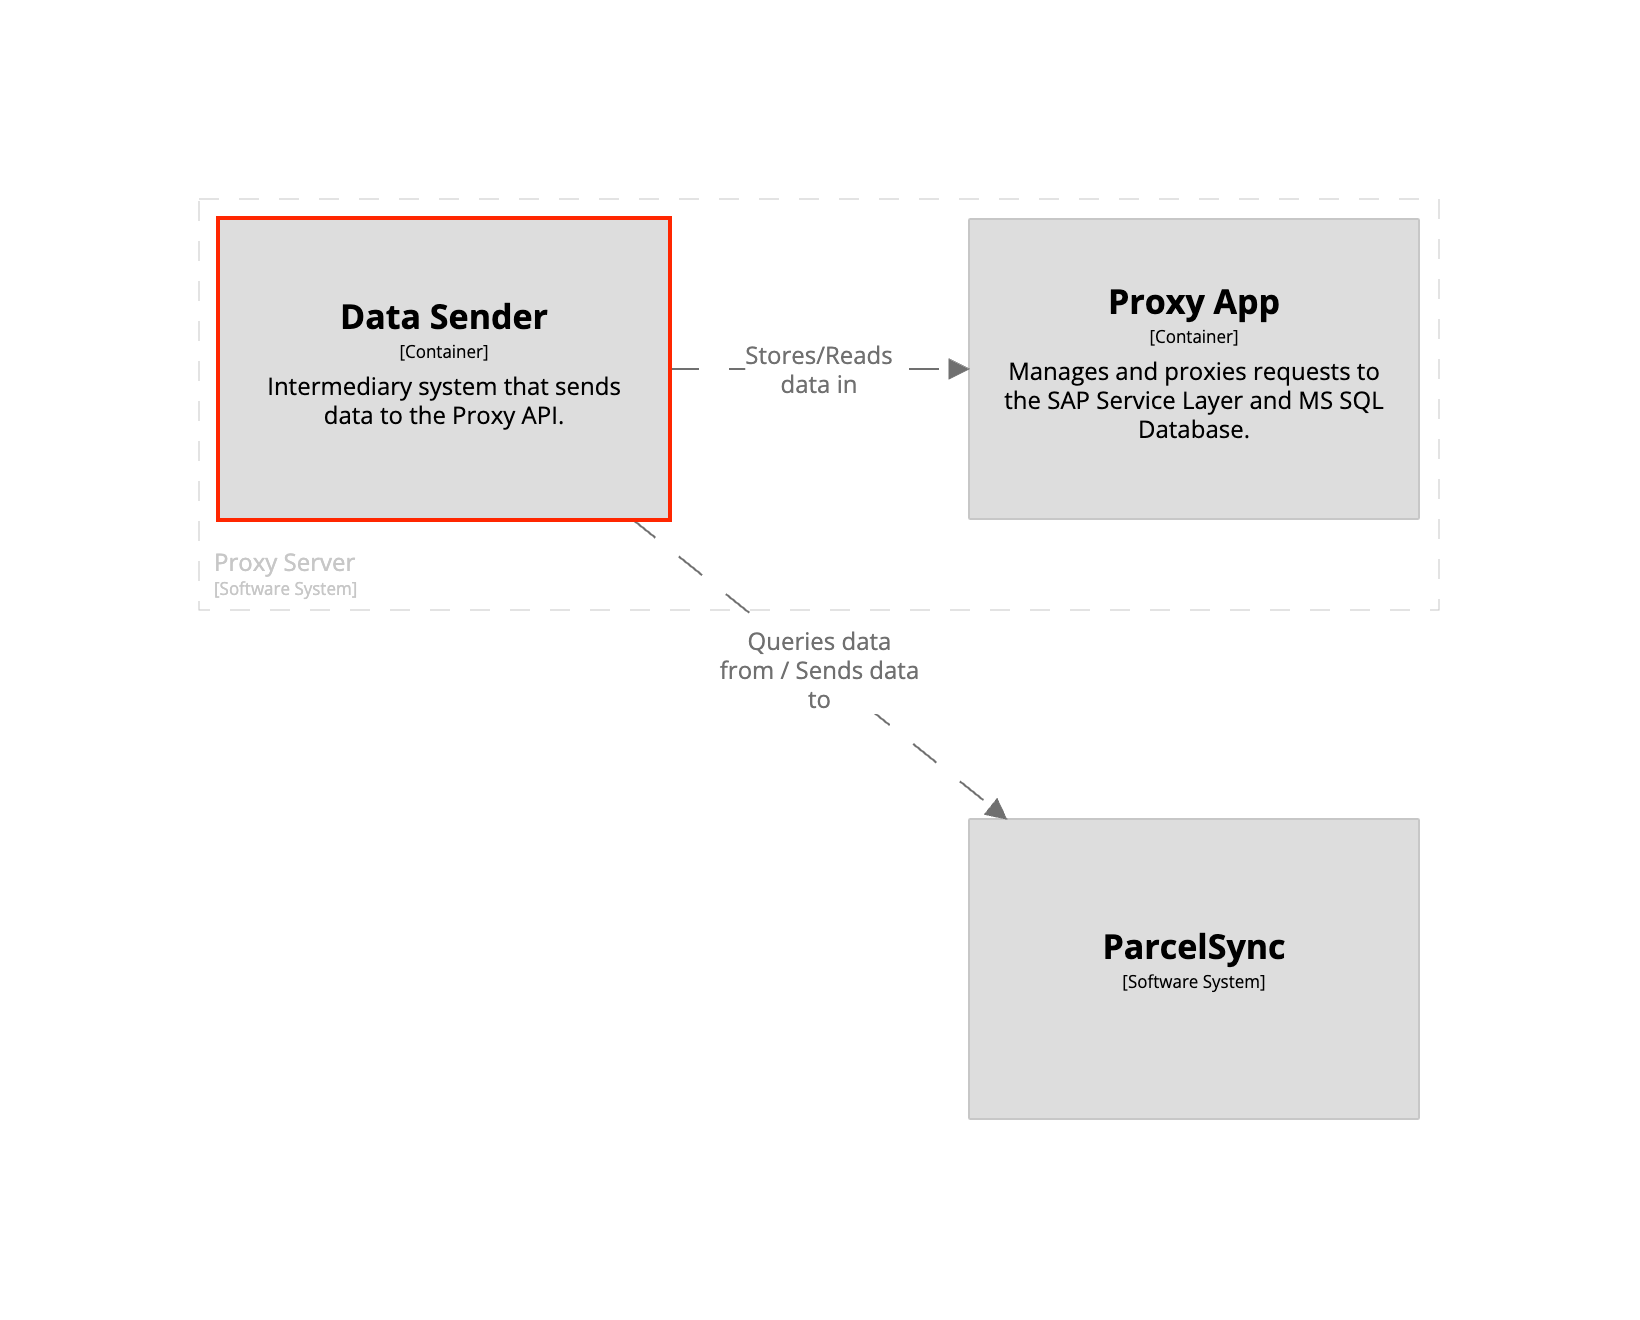
\includegraphics[width=100mm]{img/docs/fig_data_sender.png}
\caption{C4 Container diagram of \texttt{Data-sender} context}
\label{imgdocs:structurizr:data_sender}
\end{figure}

\section{Data flow}

The data flow through \texttt{Data-sender} can be generalized into two main points:
\begin{itemize}
    \item \textbf{From SAP to platform:} New and existing order details are loaded from SAP and sent to the platform. This includes orders that need platform processing and updates for existing (non-shipped) orders with modifications.
    \item \textbf{From platform to SAP:} Completed orders, including those shipped and delivered, are updated back in SAP with details such as tracking number, actual status, delivery date, and carrier specific data such as invoice number, weight, and name of the actual signed recipient.
\end{itemize}

\section{Overview}

The \texttt{Data-sender} is designed with two entry-points:
\begin{enumerate}
    \item \textbf{Scheduler:} Manages the timing of data exchange tasks, ensuring that they are executed at appropriate intervals.
    \item \textbf{\ac{CLI}:} Allows manual triggering and execution of specific scripts.
\end{enumerate}

So, the program can run in scheduled mode as well as in nonscheduled mode just by triggering the command. 

The folder structure of the program is very straight forward and defined the module separation:
\dirtree{%
.1 src.
.2 tasks.
.3 ceskaposta.
.4 new-orders.ts.
.4 update-new-orders.ts.
.4 update-old-orders.ts.
.3 packeta.
.4 new-orders.ts.
.4 update-new-orders.ts.
.4 update-old-orders.ts.
.3 ppl.
.4 new-orders.ts.
.4 update-new-orders.ts.
.4 update-old-orders.ts.
.2 types.
.3 task.ts.
.2 utils.
.3 parcelsyncApi.ts.
.3 sapApi.ts.
.2 logger.ts.
.2 setup.ts.
}

As we can see from the structure, in \texttt{src/tasks} there is a lot of redundancy in tasks.
The reason for this is that the company implementation of SAP handles each carrier slightly differently.
Due to that, the tracking numbers for the carriers are inserted into different columns and the data is fetched differently. 
Hence why, the cleanest and well maintainable approach was to implement this completely separately as isolated scripts.

\section{API fetchers}
In order to call SAP Proxy and the public API of the platform, two \texttt{AxiosInstance} were created in \texttt{src/utils/}.
Each of them calls different endpoints and handles authentication a little differently.
\begin{itemize}
    \item \textbf{\texttt{parcelsyncApi.ts}:} Defines \texttt{AxiosInstance} to call platform API with supportive scripts to generate seller identification and defines several groups of parcel statuses to help with recognition whether parcel was delivered, etc.
    \item \textbf{\texttt{sapApi.ts}:} Defines \texttt{AxiosInstance} to call SAP Proxy.
\end{itemize}

\section{Scheduler and \ac{CLI}}
All tasks available to schedule and call via \ac{CLI} are imported into \texttt{src/setup.ts} which is called from the entry \texttt{src/index.ts}.
The \texttt{setup.ts} defined a mapping for each task between the method and the standard Cron schedule definition.

Each task is then bound to the \texttt{yargs} module object as a command to run either from \ac{CLI} or as a single command triggering the scheduled mode.

\section{Carrier specific modules}
\label{subsec:programming-data-sender.carrier}

For each carrier implemented and used, there is a separate module that handles data retrieval and alteration.

Each carrier implements three main methods: 
\begin{itemize}
    \item \textbf{\texttt{new-orders}:} Queries data in SAP via SAP Proxy, transforms the data into expected format and sends to the platform. This task implements the data query with specifics for each carrier. 
    \item \textbf{\texttt{update-new-orders}:} Retrieves packages from the platform up to 1 day old and alters the tracking number, tracking link, status name and status date in SAP via SAP Proxy.
    \item \textbf{\texttt{update-old-orders}:} Retrieves parcels from the platform that are up to 20 days (\texttt{ceskaposta}, \texttt{packeta}) day old (for \texttt{ppl}, it is 35 days, more on that in Section \ref{subsec:programming-data-sender.carrier.ppl}) and alters the tracking number, tracking link, status name and status date in SAP through SAP Proxy.
\end{itemize}
\subsection{\texttt{ceskaposta}}
Implements the three standard methods as mentioned in \ref{subsec:programming-data-sender.carrier}.
\subsection{\texttt{packeta}}
Implements the three standard methods as mentioned in \ref{subsec:programming-data-sender.carrier}.
\subsection{\texttt{ppl}}
\label{subsec:programming-data-sender.carrier.ppl}

Implements the three standard methods as mentioned in \ref{subsec:programming-data-sender.carrier}, however, with some specifics to the PPL carrier.
\subsubsection{Multiple parcels in one shipment}
One specific feature of the PPL is that its API allows multi-parcel shipments. This means that we can group the data retrieved from SAP using a grouping parameter (Invoice number) and send those shipments to the platform with multiple parcels.

\subsubsection{Retrieval of Invoice number and price of the service}
Since PPL provides much more data than the two carriers mentioned above, it is possible to retrieve the PPL invoice number and the granulated cost of the shipping service. 
The platform returns these additional data obtained from tracking in \texttt{metadata} field of the status.
This can be parsed and inserted into the appropriate SAP columns in the shipment object.
Because these data are all returned on the first day of the next calendar month, it is necessary to fetch more much older shipments from the platform (hence the 35-day parameter).


